% This is samplepaper.tex, a sample chapter demonstrating the
% LLNCS macro package for Springer Computer Science proceedings;
% Version 2.20 of 2017/10/04
%
\documentclass[runningheads]{llncs}

\RequirePackage[
  % backend=bibtex,   % Recommended is `biber`, but gives
  backend=biber,     % timeout on Overleaf
  style=numeric,   % Equivalent to elsarticle-num-names
  sorting=none,    % Adjust sorting as needed
  natbib=true      % Compatibility with natbib
]{biblatex}

\usepackage{graphicx}
% \usepackage{cite}
\usepackage{url}
\usepackage{lipsum}                     % Dummytext
\usepackage{xargs}                      % Use more than one optional parameter in a new commands
\usepackage[pdftex,dvipsnames]{xcolor}  % Coloured text etc.
\usepackage{subcaption}


% Define custom colors
\definecolor{irrelevant}{RGB}{255, 0, 0} % Red color for old text
\definecolor{old}{RGB}{128, 128, 128} % Gray color for irrelevant text
\definecolor{final}{RGB}{0, 128, 0} % Green color for final text
\definecolor{edit}{RGB}{0, 0, 255} % Blue color for notes or other text


% Increase margin text width
\setlength{\marginparwidth}{2cm}

\usepackage{scrlayer-scrpage}

% Bibliography:
\addbibresource{bibliography/phd_proposal.bib}
\addbibresource{bibliography/lit_review_specific.bib}
\addbibresource{bibliography/zoom_calib.bib}

\setcounter{page}{1}


%
% ============== Define custom TODO commands ===========================
\usepackage[
  colorinlistoftodos,
  prependcaption,
  textsize=tiny,
  % disable
  ]{todonotes}

\newcommand{\comment}[2][Comment]{\todo[inline,color=blue!20!white]{\textbf{#1}: #2}}
\newcommand{\commentside}[2][Comment]{\todo[color=blue!20!white]{\textbf{#1}: #2}}
\newcommand{\fixme}[1]{%
  \todo[color=red!20, inline, size=\footnotesize]{FIXME: #1}%
}
\newcommand{\review}[1]{%
  \todo[color=blue!10, inline, size=\footnotesize]{REVIEW: #1}%
}

% With an exclamation mark icon
\newcommand{\alert}[1]{%
  \todo[inline, color=orange!30, size=\small, bordercolor=orange!80, linecolor=orange!80]{ALERT: #1}%
}

% ============== END: Define custom TODO commands ===========================

\makeatletter
\AtBeginDocument{%
  \def\doi#1{\url{https://doi.org/#1}}}
\makeatother

\makeatletter
\renewcommand\paragraph{\@startsection{paragraph}{4}{\z@}%
                                    {2.25ex \@plus1ex \@minus.2ex}%
                                    {-1em}%
                                    {\normalfont\normalsize\bfseries}}
\makeatother

%\urlstyle{same}

% Used for displaying a sample figure. If possible, figure files should
% be included in EPS format.
%
% If you use the hyperref package, please uncomment the following line
% to display URLs in blue roman font according to Springer's eBook style:
% \renewcommand\UrlFont{\color{blue}\rmfamily}

\begin{document}
%
\title{
  UGV Backtracking Recovery With Active Visual Landmarks Navigation:
  Literature Review (Assignment)
}

\author{Dmytro Kushnir\orcidID{0009-0006-8652-5781} }
%
\authorrunning{D. Kushnir}
% First names are abbreviated in the running head.
% If there are more than two authors, 'et al.' is used.
%
\institute{
  Ukrainian Catholic University, L'viv, Sventsitskogo st. 17,  79011, Ukraine
  \email{kushnir\_d@ucu.edu.ua}
}
%
\maketitle              % typeset the header of the contribution
%

\comment[]{does this type of work require "annotation" kind of block?}

\section{Introduction}

Motivation for the topic of unstructured environments is multifaceted. Industries such as agriculture, mining, and military technology require advancements in autonomous systems, yet are hindered by the lack of open-source tools.
\todo{Elaborate on why open tools are pivotal for industry advancements and research progress.}

\textbf{Problem Statement:} Defining unstructured environments and their specific challenges will provide clarity. These environments lack predefined landmarks, pose navigation difficulties, and require robust adaptable systems.
\todo{Discuss what constitutes "unstructured environments" and why they are a significant research challenge.}

\section{Methodology}
This section outlines the approach to gathering and analyzing the literature.

\subsection{Specific Traits of Domain Literature}
Research in unstructured UGV robotics exhibits several distinguishing traits:
\begin{itemize}
  \item Large-scale reviews or almanacs (aggregating 250+ papers) play a critical role in providing comprehensive overviews of the field.
  \item The volume of publications is significantly smaller than in mainstream AI, where research output is orders of magnitude higher.
  \item Research initiatives, such as DARPA and MBZIRC challenges, drive progress by clustering studies around specific problems.
  \item Long-term research is typically conducted by well-established teams with access to substantial resources.
  \item The field lacks standardized benchmarks or datasets, making cross-comparisons between studies challenging.
\end{itemize}

\subsection{Connectivity in Robotics Research}
\begin{figure}[ht]
  \centering
  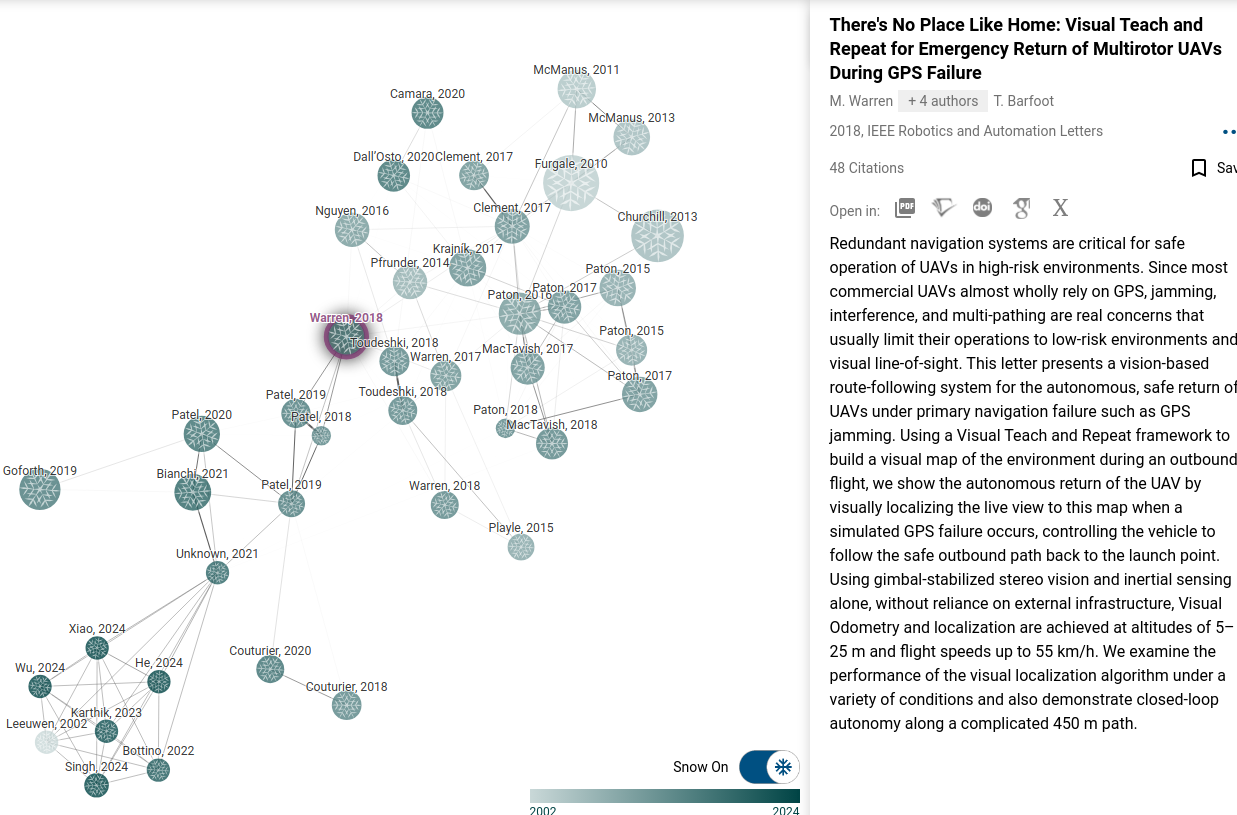
\includegraphics[width=\linewidth]{img/There_is_no_place_like_home_research_tree.png}
  \caption{Visual Teach-and-Repeat approach for emergency return of multirotor UAVs during GPS failure \cite{warren-ral19-no-place-like-Home}. More information is available on Connected Papers: \protect\url{https://www.connectedpapers.com/}.}
  \label{fig:no_place_like_home}
\end{figure}

The papers in this field are well connected, and the research is often conducted within "clusters" of research groups. An example of such clustering can be seen in the work of Warren et al. (Figure~\ref{fig:no_place_like_home}), which demonstrates the modest size but tight connections of research within this domain.

Robotics research often fragments across variables such as indoor versus outdoor environments, aerial versus ground platforms, and real-time versus non-real-time systems. Addressing these distinctions narrows the scope of each research problem, creating a "pin-tip" scale for the research frontier. With a smaller research community, large-scale benchmarks or datasets are often absent.

This fragmentation explains why research frequently focuses on specific, everyday tasks that extend beyond current robotics capabilities. One example is the "returning home" problem, a fundamental yet challenging task. Relevant papers on such tasks tend to cluster around research centers, datasets, or individual experts.

Unlike mainstream AI, which experiences terminological saturation, robotics remains more fragmented. For instance, the seminal robotics paper "FastSLAM: A factored solution to the simultaneous localization and mapping problem" (2002) has accrued approximately 3,500 citations in 20 years. In contrast, the AI paper "BERT: Pre-training of Deep Bidirectional Transformers for Language Understanding" (2018) achieved 50,000 citations in just five years. \todo{Add reference to resourses with citation statistics.}

These differences show that citation-based snowballing approaches are less effective for navigating robotics literature. Instead, comprehensive reviews, challenge-driven studies, and large-scale almanacs are better suited to understanding the field.

What matters most in this field is the careful formulation of problems and the requirements they impose. These requirements drive the system design of solutions, followed by implementation and validation. Unlike AI, where isolated benchmarks play a central role, robotics focuses on real-world conditioins versatility robustness and iterative improvements.

\comment[Here we will meticulously deconstruct the whole challange into set of requirements, investigate the available set of apporaches, tradeoffs and design the solution aspects. The CORE of literature analysis in robotics will be here. In such a manner we will ensure that we are solving the actual large-scale problem applicable beyond our setup. ]{}

\subsection{Selection Criteria}
The following criteria guided the selection of papers for this review:
\begin{itemize}
  \item Preference was given to studies with implementations adaptable to our platform or those offering detailed ground truth data demonstrations.
  \item Industry standards and widely adopted tools, especially those with robust GitHub repositories, community and versions updates were emphasized to ensure practical relevance and reproducibility.
\end{itemize}


\subsection{Analysis Framework}
The review leverages a structured "Task-Requirement-Design-Implementation-Validation" methodology.
\todo{Include visual diagrams or reference placeholders for MeROS-based design layers.}

Challenges-based research in robotics emphasizes organized progress, such as DARPA competitions, driving iterative advancements in solutions.
\todo{Amplify with examples of explosive technology disruptions, e.g., Kinect or ROS2.}

\section{State-of-the-Art}

\comment{Larger piece for ROS. Other will be detailed in similar fashion + references}

\subsection{The Critical Role of the ROS Platform}
The Robot Operating System (ROS) has emerged as a cornerstone technology in the robotics field, providing an open-source framework that standardizes development and fosters collaboration across academia and industry. Its modular architecture allows researchers and developers to integrate diverse hardware and software components, enabling rapid prototyping and scalability for a wide range of applications.

One of ROS's most significant contributions is its community-driven ecosystem, where shared libraries, tools, and documentation accelerate innovation. ROS supports real-time applications, bridging the gap between laboratory research and field deployment. This feature has proven particularly valuable in unstructured environments, where dynamic conditions demand robust and flexible solutions. Moreover, the adoption of ROS by industry leaders has enhanced its relevance, making it a platform that seamlessly connects academic research with practical deployment.

In the context of this review, ROS plays a pivotal role in the development of modular designs, such as the MeROS framework. By leveraging ROS's tools for sensor integration, motion planning, and communication, MeROS exemplifies how a standardized platform can streamline the design and validation of complex robotic systems. However, despite its strengths, ROS is not without limitations. Challenges such as real-time processing constraints, hardware compatibility, and dependency management persist, leaving room for further enhancements.

\subsection{Mapping Approaches}
Summarize current techniques in mapping for unstructured environments.
\todo{Discuss strengths and limitations of existing methods.}

\subsection{Visual Perception and PTZ Cameras}
Discuss the role of PTZ cameras in UGV platforms, emphasizing modular design and requirement-based development.
\todo{Include examples of modular designs and calibrations.}

\subsection{Public and Private SOTA}
Contrast public SOTA with proprietary solutions. Highlight the reproducibility crisis in robotics academia due to platform-locked tools.
\todo{Explore the coined term "Public SOTA" and its implications.}

\section{Research Gaps}
\subsection{Task-Requirement-Design Identification}

Core research gaps
\comment[We will concentrate our research efforts on them specifically]{}

\begin{itemize}
  \item PTZ camera integration challenges.
  \item Long-range navigation in unstructured environments:
        \begin{itemize}
          \item Representation of places.
          \item Route following between places with minimal memorization.
        \end{itemize}
  \item Encapsulation of independent software-hardware modules.
  \item Cross-platform interfacing and requirements management.
  \item Calibration and processing for open-source tools.
\end{itemize}
\todo{Explore solutions like 360-degree cameras or alternative configurations.}

\subsection{Constraints and Challenges}
\comment[Those are factors that can have decisive impact on feasibility of the work and they require our attention, but those fell out of the main focus of the research]{}

\begin{itemize}
  \item Planning and power management.
        Long-range navigation is limited by the energy capacity of the UGV and the efficiency of its spending.
  \item Environmental factors such as weather, light, and terrain complexity.
        This parameter has to be mentioned, to clearly denote limitations of considered conditions.
  \item Real-time processing requirements.
        The real-time processing of sensor data and decision-making are important for the robotisc, but we outline the problem and design solution in such a manner to allow for the relaxations on this requirement.
  \item Scalability and integration with ROS platforms.
        As we touch lots of system aspects with limited resources, we will focus on the iterative implementations and open solutions.
\end{itemize}
\todo{Discuss relaxations on real-time requirements and focus on iterative implementations.}

\section{Conclusion and Motivation}
The proposed research aims to:
\begin{itemize}
  \item Emphasize modular design and cross-platform usability.
  \item Identify critical bottlenecks halting advancements.
  \item Validate the feasibility of addressing these bottlenecks through:
        \begin{itemize}
          \item Open-source calibration and integration tools.
          \item Testing on Husky UGV or equivalent platforms.
          \item Clear documentation and interfaces following MeROS philosophy.
        \end{itemize}
\end{itemize}
\todo{Highlight the significance of open-source contributions and iterative validation in advancing the field.}

\section{Datasets and Resources}
A few datasets can serve as a basis for this research or as a sign of missing data:
\begin{itemize}
  \item Wild Scenes Dataset: \url{https://arxiv.org/pdf/2404.18477}
  \item Wild Places Dataset: \url{https://csiro-robotics.github.io/Wild-Places}
  \item Freiburg Forest: \url{https://paperswithcode.com/dataset/freiburg-forest}
\end{itemize}
\todo{Note the gaps in available datasets and propose directions for addressing these limitations.}


\printbibliography


\end{document}
```
